\chapter{Summary and conclusion} %%%%%%%%%%%%%%%%%%%%%%%%%%%%%%%%%%%%%%%%%%%%%%%%%%%%%%%%%%%%%%%%%
\label{chap:conclusion} %%%%%%%%%%%%%%%%%%%%%%%%%%%%%%%%%%%%%%%%%%%%%%%%%%%%%%%%%%%%%%%%%%%%%%%%%%

- Write a little about the current state of neutrino physics and current planed experiments as a
intro to the conclusion!
- Talk about it all in the past tense, definitely the best way to do this chapter!

1) Motivate the need for \chips and explain how it accomplishes its aims
    - Use readily available bodies of water of the earths surface
    - Provides a dramatic reduction in cost per kt of sensitive mass to between \$200k-\$300k
    - No excavation
    - Commercially available components wherever possible
    - Easy to build, quick to deploy, and upgradable once operational
    - Multiple detector modules can be flexibly combined depending on available resources
    - Only use accelerator beam neutrinos, optimised instrumentation coverage
    - Standard construction materials, stainless steel and PVC, using modular POMs
    - Commercially available cheap filtration for adequate water attenuation lengths
    - Although \chipsfive has not been fully proven yet, future \chips detectors will continue to
    prototype the concept
    - A DAQ system in line with the core concepts of \chips has also been developed for \chipsfive
    again testing the use of commercially available components both hardware and software, proving
    successful. 
    - Particularly the use of open source software rather than bespoke components, the years of
    using fully bespoke components should really come to an end.

2) Show that CNNs can be used to fully reconstruct and classify neutrino events within water
Cherenkov detectors and provide significant performance improvements on standard methods whilst
doing so. At the same time as being explainable and robust, which are of course a key concern of
any new methodology or approach. 
    - Can all be done incredibly quickly rather than multiple long running algorithms can just run
    very fast inference of a few networks.
    - Less reliance on heavily human influenced bespoke software frameworks
    - Sufficient cosmic rejection for negligible beam sample contamination is achieved
    - Beam classification selection is surprisingly comparable to other costly experiments
    - Energy estimation is comparable and more generalisable compared to standard methods
    - Cherenkov ring and Hough peak features are clearly being learnt by the trained networks
    - There is clear learnt separation between categories as seen via unsupervised methods
    - The smearing of hit times is found to have a negligible impact on performance
    - Robust to charge calibration
    - Random PMT noise is found to have a negligible impact on performance

3) Inform the application of CNNs to other similar water Cherenkov detectors in the future. 
    - Viewing the event from interaction vertex position is clearly the most promising view
    - The training sample must match the expected composition of events closely
    - The network architecture does not matter much in the context of this work
    - Multitask learning is shown to provide increased performance and should be further explored
    - Explore larger input image sizes and network architectures
    - Study the input distribution of events in greater detail
    - Look at using a graph convolutional network or transformers ;)
    - Exploit the ability to separate exclusive final states (particle counting) to increase 
    - Look at fiducial cut and understand if upstream beam events will be a problem
    - Flat energy spectrum for energy estimation training sample
    - Train beam classification network on only contained events
    - Other methods to reduce distortions, such as the smearing of hits across nearby bins to   
    reduce isolated peaks and an improved interaction vertex position estimation.
    - use of a different loss function to promote learning for the less common interaction types 
    and to maximise the physics sensitivity rather than simply accuracy
    - The real power of such techniques is still not fully understood, and only time will tell
    what additional impact they may have within neutrino physics.

- It is now abundantly clear that convolutional neural networks will play a key role in the event
reconstruction and classification for \chips. What is also clear is that other water Cherenkov
neutrino experiments, which up to now have not fully embraced modern machine learning techniques
as much as other sectors of the neutrino field should do so. For a range of benefits from
increased processing time, leverage the wider computer vision ML field to make the advancements
for you while you focus on the physics analysis.

\begin{figure} % CHIPS RAMP DIAGRAM %
    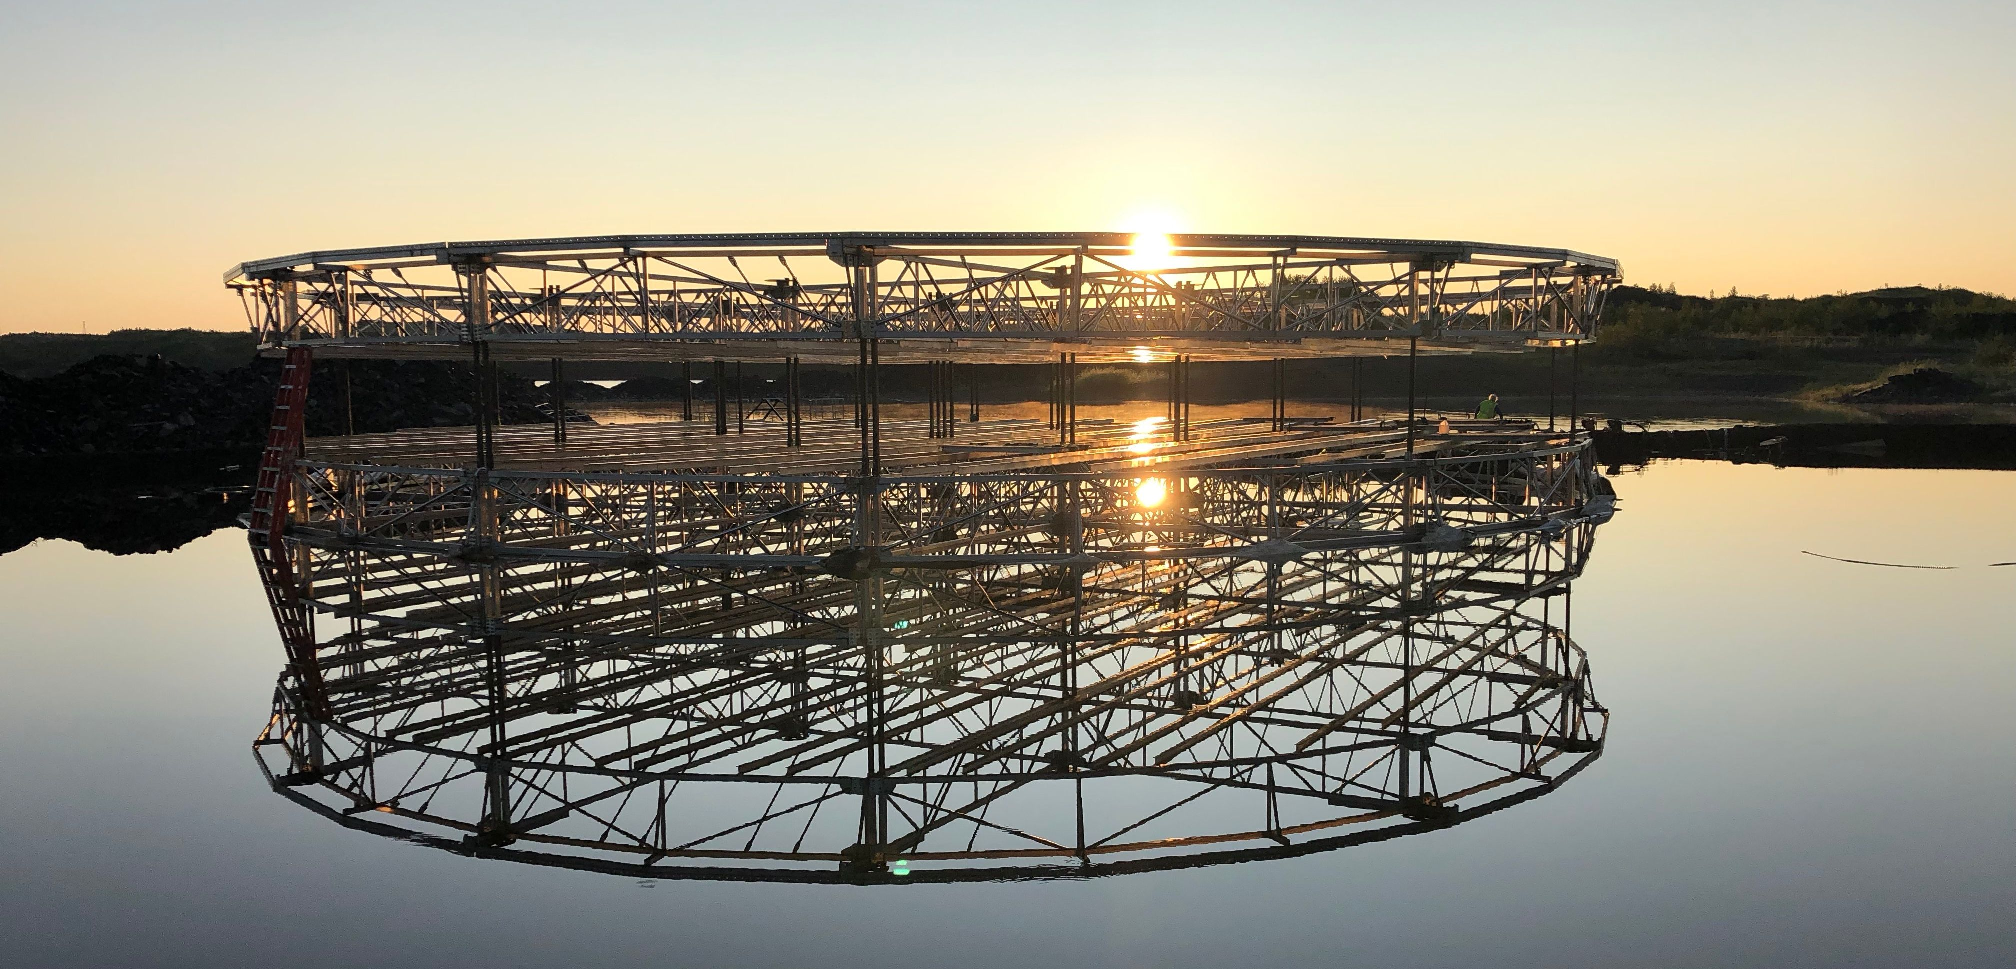
\includegraphics[width=\textwidth]{diagrams/4-chips/sunrise.pdf}
    \caption*{The \chipsfive detector frame at sunrise.}
\end{figure}